\section{Auswertung}

\subsection{Pockelseffekt}

\subsubsection{Sinusmodulation}

Wir haben zwei getrennte Messreihen à ca. 15 Messpaaren aufgenommen. Ein Messpaar bestand daraus, sowohl bei positiver als auch bei negativer Spannung, den Wert der Gleichspannung zu finden, bei dem das Sinussignal mit doppelter Frequenz am besten sichtbar war.

Messreihe 1 wurde bei $2010 \pm 7 Hz$ Sinussignal aufgenommen, Messreihe 2 bei $1800 \pm 1 Hz$ bzw $1815 \pm 1 Hz$ aufgenommen. Der Frequenzgenerator zeigte bei Messreihe 1 einen Drift von ca. $2017 Hz$ auf $2003 Hz$, blieb aber bei Messreihe 2 bis auf kleine Schwankungen stabil. Die Frequenzänderung bei Messreihe 2 ergibt sich dadurch, dass wir die Messung für eine Mittagspause unterbrochen haben.

\begin{python}
from numpy import *

from numbers import *

def sinus_auswertung(u_plus, u_minus):
  u_halb = [u_plus[i] + u_minus[i] for i in range(len(u_plus))]

  print '\n'

  print r'\begin{tabular}{rrr} \toprule'
  print r' $U_+$ [V] & $U_i$ [V] & $U_{\lambda/2}$ [U] \\'
  print r' \midrule '

  for i in range(len(u_plus)):
    print r'{u_plus:> 5.1f}&{u_minus:> 5.1f}&{u_halb:> 5.1f}\\'.format(u_plus=u_plus[i], u_minus=-u_minus[i], u_halb=u_halb[i])

  print r'\bottomrule '
  print r'\end{tabular}'
  print '\n'
  print '\n'

  u_halb_a = array(u_halb)
  print '\n'
  #print r'Anzahl: {anzahl} \\'.format(anzahl = len(u_halb_a))
  #print r'Summe: {summe:.5f}\\'.format(summe = sum(u_halb_a))
  u_l2 = mean(u_halb_a)
  s_u_l2 = std(u_halb_a)
  print r'$U_{\lambda/2} = $', n_e_to_latex(u_l2, s_u_l2, 1, 0), 'V \n' 
  
  return u_l2, s_u_l2

  

u_plus_r  = [164.1, 162.4, 161.9, 161.9, 162.3, 158.2, 156.3, 156.0, 156.1, 156.6, 155.2, 154.7, 152.5, 151.2, 151.4, 150.3]
u_minus_r = [89.9, 90.6, 90.4, 90.2, 91.9, 92.9, 93.4, 93.3, 92.8, 93.4, 94.0, 94.6, 97.3, 98.3, 99.3, 99.4]

u_plus_s = [153.6, 155.6, 156.7, 156.7, 157.5, 155.3, 154.9, 156.0, 154.3, 153.7, 154.2, 154.8, 154.1, 154.8, 154.8]
u_minus_s = [99.9, 99.5, 98.6, 97.4, 98.6, 97.9, 100.4, 100.3, 104.0, 103.6, 103.8, 104.3, 104.6, 104.1, 104.3]  


print r'''\begin{table}[H]
\begin{minipage}[b]{0.5\linewidth}
\centering
         '''

u_l2_r, s_u_l2_r = sinus_auswertung(u_plus_r, u_minus_r)

print r'''  \caption{Messreihe von Robi}
	  \end{minipage}
	  \begin{minipage}[b]{0.5\linewidth}
	    \centering
           '''

u_l2_s, s_u_l2_s = sinus_auswertung(u_plus_s, u_minus_s)


print r'''\caption{Messreihe von Simon}
	  \end{minipage}
          \end{table} '''

print r'Daraus k\"onnen wir nun $r_{41}$ berechnen:'

print r'$$ r_{41} = \frac{\lambda d}{4l U_{\lambda / 2}} \left(  \sqrt{\frac{1}{2} \left( \frac{1}{n_1^2} + \frac{1}{n_3^2} \right)} \right)^3 $$'

print 'sowie den Fehler: '

print r'$$S_{r_{41}} = r_{41} \frac{S_{U_{\lambda/2}}}{U_{\lambda/2}} $$'

lmbd = 632.8e-9 #m
d = 2.4e-3 #m
l = 20.0e-3 #m
n1 = 1.522
n3 = 1.477

print r'''Die Werte f\"ur\\
Wellenl\"ange $\lambda$ = ''' + number_to_latex(lmbd, 1, -9) + r'''nm \\
Kristalldicke d = ''' +number_to_latex(d, 1, -3) + r'''m\\
Zellenl\"ange l = ''' + number_to_latex(l, 1, -3) + r'''m\\
Brechungsindex 1 $n_1$ = ''' + repr(n1) + r'''m\\
Brechungsindex 3 $n_3$ = ''' + repr(n3) + r'''m\\
sind in der Versuchsanleitung gegeben und werden von uns als fehlerfrei idealisiert.
'''

def r_41(lmbd, d, l, U, n1, n3):
  return d*lmbd/(4.0*l*U)*(0.5*(1/(n1**2) + 1/(n3**2)))**(1.5)

r_41_r = r_41(lmbd, d, l, u_l2_r, n1, n3)
s_r_41_r = r_41_r * s_u_l2_r / u_l2_r
r_41_s = r_41(lmbd, d, l, u_l2_s, n1, n3)
s_r_41_s = r_41_s * s_u_l2_s / u_l2_s

print r'''Somit erhalten wir die Ergebnisse:\\
\begin{center}
\fbox{
'''

print r'$r_{41_r} = $', n_e_to_latex(r_41_r, s_r_41_r, 3, -12), r' pm/V\\'
print r'$r_{41_s} = $', n_e_to_latex(r_41_s, s_r_41_s, 3, -12), r' pm/V\\'

print r'''
}
\end{center}
'''

\end{python}

Zum Vergleich, der Literaturwert beträgt: $r_{41} = 23.4 pm/V$

\subsubsection{Sägezahnmodulation}

\begin{figure}[H]
 \centering
 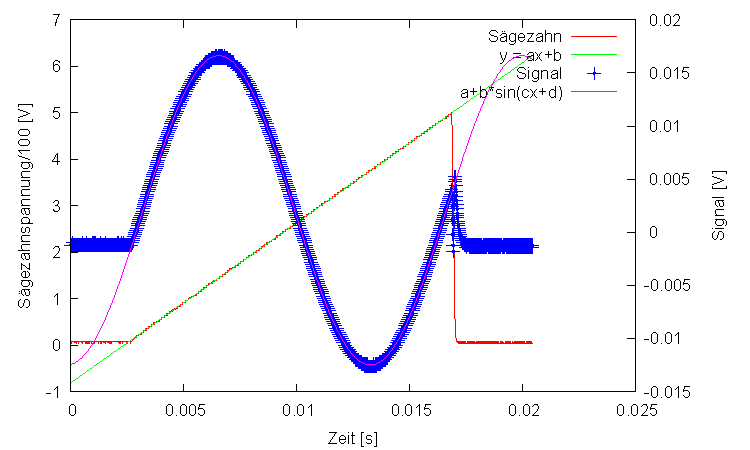
\includegraphics{messwerte/saegezahn/saegezahn_1.pdf}
 \caption{Sinusförmiges Signal als Reaktion auf eine Sägezahnspannung}
\end{figure}

Wir haben die Pockelszelle mit der Spannung eines Sägezahngenerators betrieben und konnten auf dem Oszilloskop einen sinusförmigen Verlauf der Intensität des Photodiodensignals beobachten. Über eine lineare Regression der ansteigenden Spannungsflanke berechnen wir $\frac{\Delta U}{\Delta t}$ und können somit aus der halben Periodendauer des Sinussignals auf die Halbwellenspannung $U_{\lambda/2}$ schliessen. Da die Sägezahnspannung bis zu 500V erreicht und der Oszilloskop diese nicht abbilden kann, wird das Signal mit einem Dämpfer reduziert. Um diesen Dämpfungsfaktor zu bestimmen, haben wir die doppelte Amplitude eines Sinussignals einmal mit Dämpfung $2U_D = 2.080V$ und einmal ohne $2U_{OD} = 220.00V$ gemessen.

Der Dämpfungsfaktor beträgt also
$$ D = \frac{2U_OD}{2U_{D}} = 105.769 $$

Für die lineare Regression haben wir
$$ U_{saege}(t) = a  t + b $$
und für den Fit des Signals
$$ U_{sinus}(t) = \mathit{amp}  \sin(\mathit{fr} t + \mathit{ph}) + \mathit{off} $$
verwendet. Die Halbwellenspannung erhalten wir nun über
$$ U_{\lambda/2} = \frac{1}{2}\frac{D a 2 \pi}{ fr} =  \frac{D a \pi}{fr} $$
und somit $r_{41}$ über die schon bekannte Gleichung
$$ r_{41} = \frac{\lambda d}{4l U_{\lambda / 2}} \left(  \sqrt{\frac{1}{2} \left( \frac{1}{n_1^2} + \frac{1}{n_3^2} \right)} \right)^3 $$


\begin{python}
from numbers import *
from math import pi, sqrt

#Daempfungsfaktor
D = 105.76923076923076

lmbd = 632.8e-9 #m
d = 2.4e-3 #m
l = 20.0e-3 #m
n1 = 1.522
n3 = 1.477

def r_41(lmbd, d, l, U, n1, n3):
  return d*lmbd/(4.0*l*U)*(0.5*(1/(n1**2) + 1/(n3**2)))**(1.5)

def saege(a, sa, fr, sfr):
  U = a * D / fr * pi #nur eine halbe periode
  sU = U * sqrt((sa/a)**2+(sfr/fr)**2)
  r = r_41(lmbd, d, l, U, n1, n3)
  sr = r * sU /U
  print r' ', n_e_to_latex(a, sa, 3, 0), r' & ', n_e_to_latex(fr, sfr, 3, 0), r' & ', n_e_to_latex(U, sU, 3, 0), r' & ', n_e_to_latex(r, sr, 3, -12), r'\\', '\n'
  return r

print r'''\begin{table}[H]
 \centering
 \begin{tabular}{llll}
  \toprule
  a [V/s]  &  fr [ $s^{-1}$] & $U_{\lambda/2}$ [V] & $r_{41} [pm/V]$ \\
  \midrule
'''
rges = 0
rges += 0.2 * saege(a= 343.879, sa = 0.0852, fr = 467.743, sfr = 0.0723)
rges += 0.2 * saege(a = 343.848, sa = 0.08643, fr = 467.484, sfr = 0.07867)
rges += 0.2 * saege(a = 344.282, sa = 0.08705, fr = 467.366, sfr = 0.08143)
rges += 0.2 * saege(a = 344.323, sa = 0.08556, fr = 467.776, sfr = 0.07919)
rges += 0.2 * saege(a = 344.323, sa = 0.08556, fr = 467.776, sfr = 0.07919)

sr = 7.0e-15/sqrt(5.)

print r'''
\bottomrule

\end{tabular}
\caption{Ergebnisse S\"agezahn}
\end{table}

Wir erhalten also den Mittelwert

$r_{41} = $''' +  n_e_to_latex(rges, sr, 3, -12) + r''' pm/V'''

\end{python}



\subsection{Faradayeffekt}

Messung von $2\epsilon$:
$\alpha_1 = 8.4$

$\alpha_2 = 174,8$

\newcommand{\faradayDesc}{
Wir berechnen das Magnetfeld auf der Achse:

und integrieren darüber
$\int H dl$

Vergleich mit $ H = \frac{N I}{l} $

Berechnen die Verdetkonstante

$$ \alpha = l V H $$

Wir führen eine lineare Regression durch und erhalten die Steigung $a$ und den Achsenabschnitt $b$.

Es gilt $$ \alpha = V \int H(z) dz= V 2556 I = a I + b $$

Der Achsenabschnitt $b$ enthält den Offset bei der Winkelmessung und ist nicht weiter von Bedeutung.

Somit erhalten wir die Verdetkonstante aus $$ V = \frac{a}{2556} $$  

}

\begin{python}
from scipy import stats
from math import *

from numbers import *

def auswertung_faraday(I, s_I, alpha, s_alpha):
  for i in range(len(alpha)):
    if alpha[i] > 100:
      alpha[i] = alpha[i]-180.0

  print '\n'

  print r'\begin{tabular}{rr} \toprule'
  print r' I [A] & $\alpha$ [$\circ$] \\'
  print r' \midrule '

  for i in range(len(I)):
    print r' {I:> 7.3g}  &  {alpha:> 7.3g} \\ '.format(I = I[i], alpha = alpha[i])

  print r'\bottomrule '
  print r'\end{tabular}'
  print '\n'
  print '\n'

  (a,b,r,tt,stderr)=stats.linregress(I, alpha)

  print r'Steigung: ' + n_to_latex(a, 3, 0) + '\n'
  print r'Achsenab: ' + n_to_latex(b, 3, 0) + '\n'

  return a, b


I_s = [-0.01, 0.5, 1.0, 1.5, 2.0, 2.5, 3.0, 3.5, 4.0, 4.47, +0.01, -0.5, -1.0, -1.5, -2.0, -2.5, -3.0, -3.5, -4.01, -4.50]
alpha_s = [0.50, 179.80, 178.05, 176.25, 175.42, 174.41, 173.10, 171.80, 170.48, 169.0, 0.55, 2.25, 3.40, 4.60, 5.85, 7.10, 8.40, 9.50, 10.80, 12.01]

I_r = [0.01, 0.5, 1.0, 1.5, 2.0, 2.5, 3.0, 3.5, 4.01, 4.52, -0.01, -0.51, -1.0, -1.5, -2.0, -2.49, -3.0, -3.5, -4.01, -4.53]
alpha_r = [0.35, 179.15, 177.9, 176.3, 175.0, 174.05, 172.65, 171.60, 170.25, 168.85, 0.40, 1.70, 3.10, 4.50, 5.55, 7.00, 8.25, 9.40, 10.80, 12.15]

s_I = 0.01
s_alpha = 0.004


print r'''\begin{table}[H]
\begin{minipage}[b]{0.5\linewidth}
\centering
         '''
a_s_s, b_s_s = auswertung_faraday(I_s, s_I, alpha_s, s_alpha)

print r'''  \caption{Messreihe von Simon}
	  \end{minipage}
	  \begin{minipage}[b]{0.5\linewidth}
	    \centering
           '''

a_s_r, b_s_r = auswertung_faraday(I_r, s_I, alpha_r, s_alpha)

print r'''\caption{Messreihe von Robi}
	  \end{minipage}
          \end{table} '''




print r'''\faradayDesc'''

V_s = a_s_s/2556
SV_s = V_s * sqrt((s_alpha)**2 + (s_I)**2)

V_r = a_s_r/2556
SV_r = V_r * sqrt((s_alpha)**2 + (s_I)**2)

u = 0.6*79.59

print r'''
\begin{table}[H]
\begin{tabular}{rrrr}
 \toprule
 Steigung $a$ [${}^{\circ}/A$] & Achsenabschnitt $b$ [${}^{\circ}$] & Verdetkonstante $V$ [${}^{\circ}/A$] & $V$ [$min/Oe \cdot cm$] \\
 \midrule
''' + str(round(a_s_s, 3))+ r' & ' + str(round(b_s_s, 3)) + r' & ' + number_error_to_latex(V_s, SV_s, 2, -6) + r' & ' + n_e_to_latex(V_s*u, SV_s*u, 5, 0) + r'''\\
''' + str(round(a_s_r, 3))+ r' & ' + str(round(b_s_r, 3)) + r' & ' + number_error_to_latex(V_r, SV_r, 2, -6) + r' & ' + n_e_to_latex(V_r*u, SV_r*u, 5, 0) + r'''\\
 \bottomrule  
\end{tabular}
\caption{Ergebnisse der Untersuchung des Faradayeffekts}
\end{table}

'''

\end{python}

Laut Herstellerangaben beträgt die Verdetkonstante des Flintglasstabes $V = 0.05 \frac{min}{Oe \cdot cm}$. Unsere beiden Messergebnisse bestätigen diese Angabe auch relativ gut.

\paragraph{Anmerkung}
Die Umrechnung von $\frac{{}^{\circ}}{A}$ zu $\frac{min}{Oe \cdot cm}$ ist:
$$ 1 {}^{\circ} = 60 min $$
$$ 1 A = \frac{100}{79.59}Oe \cdot cm $$
und somit
$$ 1 \frac{{}^{\circ}}{A} = 0.6 \cdot 79.59  \frac{min}{Oe \cdot cm} $$
